\documentclass{beamer}
\mode<presentation>
{
\usetheme{CambridgeUS}
\usecolortheme{beaver}
}

\usepackage[numbers]{natbib}
\usepackage{url}
\usepackage{kotex}
\usepackage{hyperref}
\usepackage{multirow}
\usepackage{graphicx}
\usepackage{amssymb,amsfonts,amsmath}
\usepackage{booktabs}
\usepackage{colortbl}
\usepackage{cite}
\usepackage[labelfont=bf,labelsep=period,justification=raggedright]{caption}
%\usepackage{subcaption}
\usepackage[caption = false]{subfig}
\usepackage{color}

\newcommand{\pkg}[1]{{\normalfont\fontseries{b}\selectfont #1}} 
\let\proglang=\textit
\let\code=\texttt 

\ifdefined\knitrout
  \renewenvironment{knitrout}{\begin{footnotesize}}{\end{footnotesize}}
\else
\fi

\AtBeginSection[]
{
   \begin{frame}
       \frametitle{Contents}
       \tableofcontents[currentsection]
   \end{frame}
}


\begin{document}


\title{ \textbf{딥러닝(Deep Learning)} }
\subtitle{\textbf{역사와 현재, 그리고 보건학으로의 적용}}
\author{\textbf{김진섭}}
\institute{서울대 보건대학원}
\date{\today}
\begin{frame}
\titlepage
\end{frame}

\section{\protect\textbf{What is Deep Learning?}}
\begin{frame}{Machine Learning}
\begin{itemize}
\item 컴퓨터가 학습하여 예측할 수 있도록 예측모형(prediction)을 개발하는 인공지능의 한 분야.
\item Computer science + Statistics ??
\item Amazon, Google, Facebook..
\end{itemize}
\end{frame}


\begin{frame}{Neural Network}
\textbf{Human brain} VS \textbf{Computer}
\begin{itemize}
\item $3431 \times 3324 = ?? $
\item 개와 고양이 구별, 음성인식, 문자인식  
\end{itemize}
\textbf{Sequential} VS \textbf{Parallel} 
\end{frame}

\begin{frame}{Neuron \& Artificial Neural Network(ANN)\citep{maltarollo2013applications}}
\begin{figure}
\includegraphics[width=3in]{/home/secondmath/Dropbox/GSPH/myreview/ml/neural1.png}
\caption{(A) Human neuron; (B) artificial neuron or hidden unity; (C) biological synapse; (D) ANN synapses.}
\end{figure}
\end{frame}

\begin{frame}
\begin{figure}
\includegraphics[width=4in]{/home/secondmath/Dropbox/GSPH/myreview/ml/neural2.png}
\end{figure}
\url{http://www.nd.com/welcome/whatisnn.htm}
\end{frame}

\begin{frame}
\begin{figure}
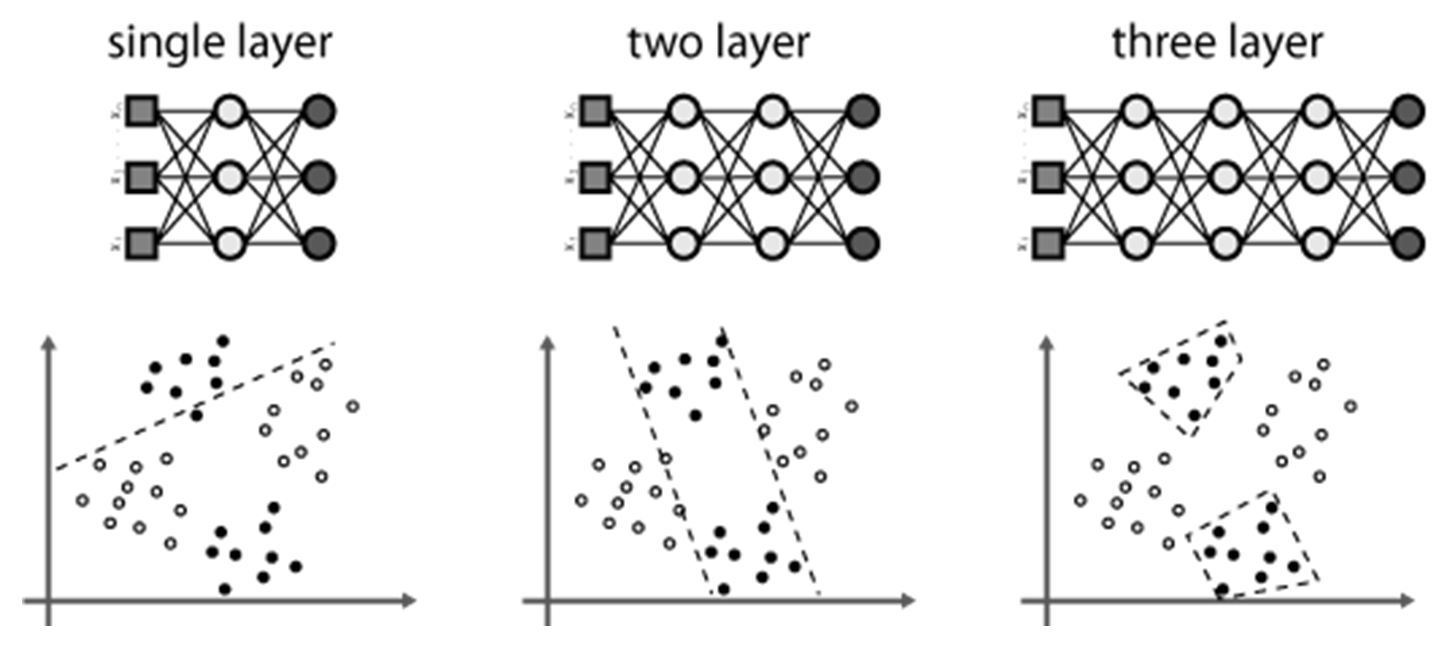
\includegraphics[width=4in]{/home/secondmath/Dropbox/GSPH/myreview/ml/neural3.jpg}
\end{figure}
\textbf{Deep Neural Network(DNN)} $\simeq$ \textbf{Deep Learning}
\end{frame}



\begin{frame}
\begin{itemize}
\item \textbf{글로벌 IT기업 `기계학습' 집중} \url{http://www.dt.co.kr/contents.html?article_no=2014062002010960718002}
\item \textbf{세계는 지금 인공지능 열풍 6조달러 블루오션 한국은 `꽝'} \url{http://vip.mk.co.kr/news/view/21/20/1178659.html}
\item \textbf{MS 클라우드, `머신러닝'으로 똑똑해진다} \url{http://www.bloter.net/archives/196341}
\item \textbf{떠오르는 5대 주요 기술과 `딥러닝'} \url{http://www.wikitree.co.kr/main/news_view.php?id=157174}
\item \textbf{인공지능 시대 구글의 맨해튼 프로젝트} \url{http://weekly.chosun.com/client/news/viw.asp?nNewsNumb=002311100009\&ctcd=C02}
\end{itemize}
\end{frame}





\section{\protect\textbf{History}}
\subsection{Perceptron}
\begin{frame}{Perceptron}
\textbf{1958년 Rosenblatt}\citep{rosenblatt1958perceptron}.

\begin{align}
y=\varphi(\sum_{i=1}^n w_ix_i+b)
\end{align}
($b$: bias, $\varphi$: activation function(e.g: logistic or $tanh$))

\begin{figure}[!ht]
\centering
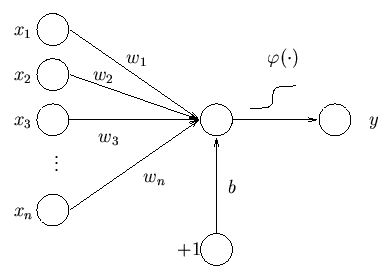
\includegraphics[width=2.2in]{/home/secondmath/Dropbox/GSPH/topic_review/DNN/perceptron.png}
\caption{\bf {Concept of Perceptron\citep{perceptronfig}}}
\label{perceptron1}
\end{figure}
\end{frame}

\begin{frame}{Low Performance}
\textbf{XOR도 해결하지 못한다}\citep{perceptroncant}.
\begin{figure}[!ht]
\centering
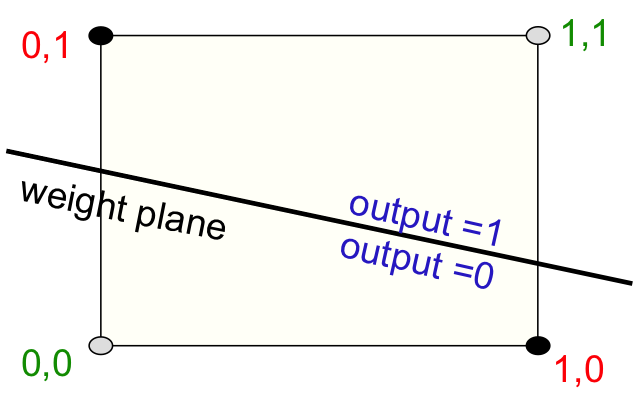
\includegraphics[width=3in]{/home/secondmath/Dropbox/GSPH/topic_review/DNN/notperceptron.png}
\end{figure}
\end{frame}


\subsection{Multilayer Perceptron}
\begin{frame}{Multilayer Perceptron}
\textbf{Hidden layer를 늘리면 해결된다!!}
\begin{figure}
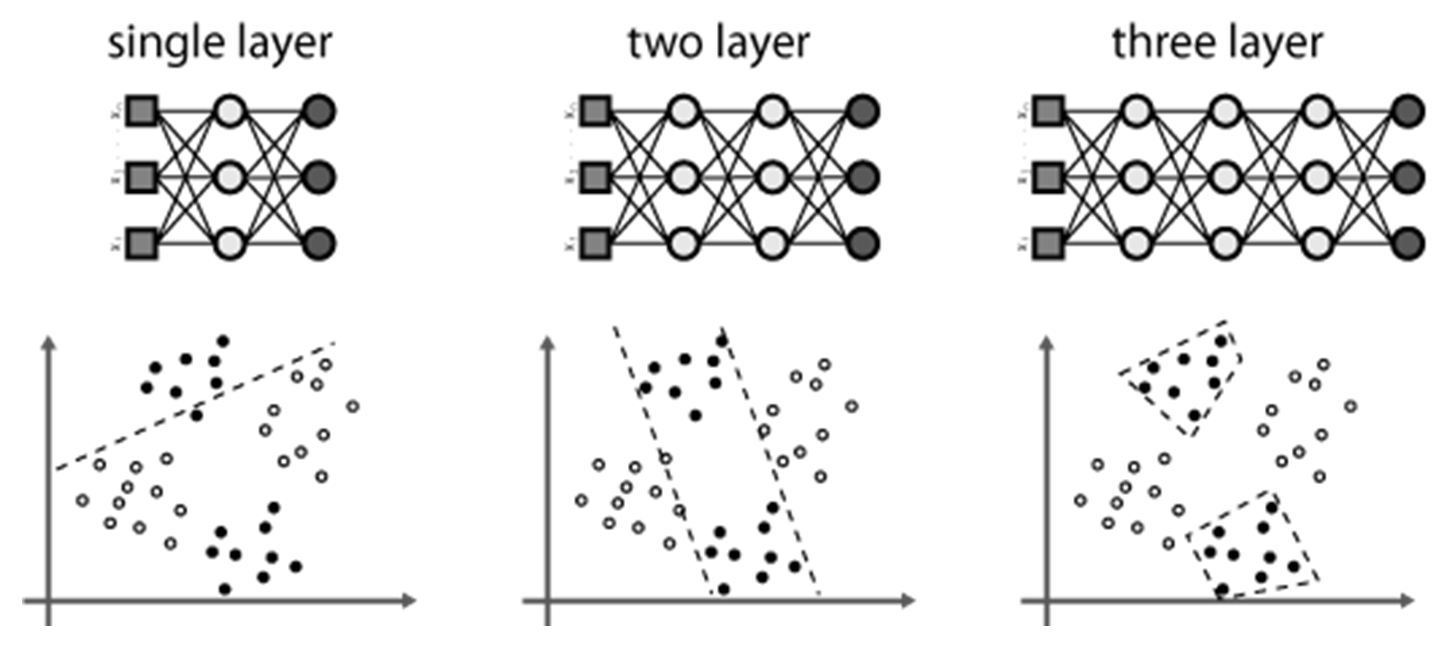
\includegraphics[width=4in]{/home/secondmath/Dropbox/GSPH/myreview/ml/neural3.jpg}
\end{figure}
\end{frame}

\begin{frame}{Learing Problem}
\begin{itemize}
  \item Hidden layer증가 $\rightarrow$ Weight 갯수 증가..
  \item 1985년: \textbf{Error Backpropagation Algorithm}\citep{rumelhart1985learning}
  \begin{itemize}
   \item Gradient Descent Methods
   \item 뒤에서부터 거꾸로..
  \end{itemize}
\end{itemize}
\end{frame}

\begin{frame}{Gradient Descent Methods}
\textbf{Weight 갯수가 너무 많다..}
\begin{itemize}
  \item Linear regression: Least square, maximum likelihood: Exact calculation.
  \item MLP: \textbf{No exact method}
\end{itemize}
\end{frame}

\begin{frame}{Gradient Descent Algorithm\citep{gradient}}
\begin{figure}
\centering
\subfloat[Large Gradient]{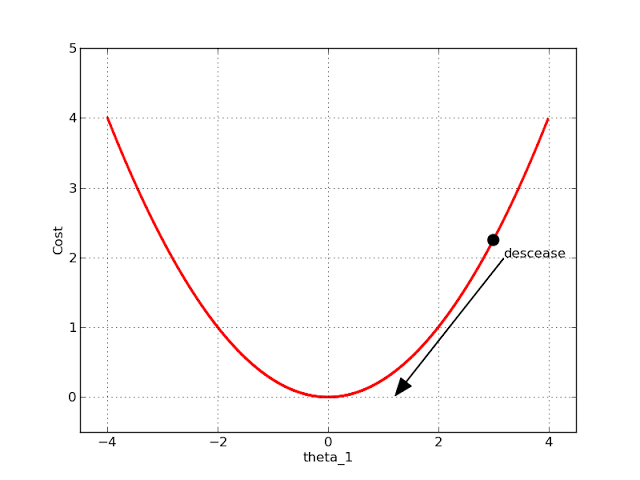
\includegraphics[width = 1.5in]{/home/secondmath/Dropbox/GSPH/topic_review/DNN/hy1.png}} 
\subfloat[Small Gradient]{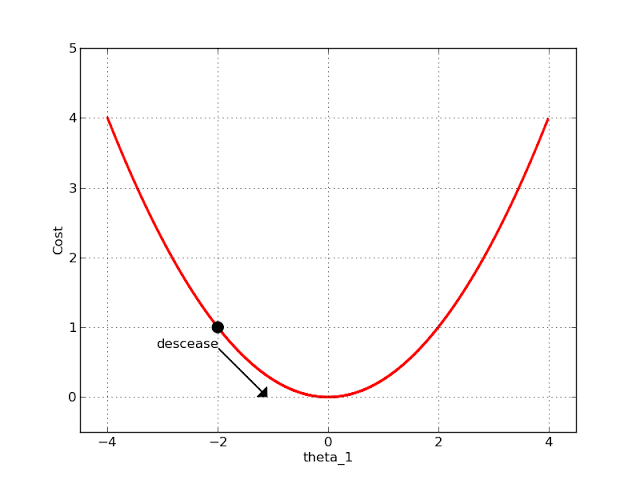
\includegraphics[width = 1.5in]{/home/secondmath/Dropbox/GSPH/topic_review/DNN/hy2.png}}\\
\subfloat[Small Learning Rate]{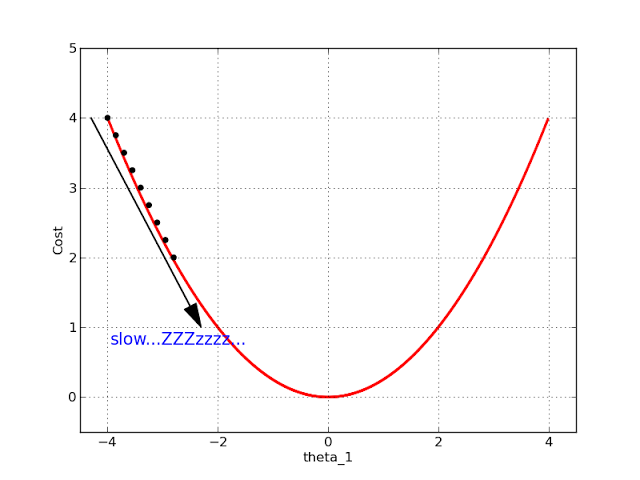
\includegraphics[width = 1.5in]{/home/secondmath/Dropbox/GSPH/topic_review/DNN/hy3.png}}
\subfloat[Large Learning Rate]{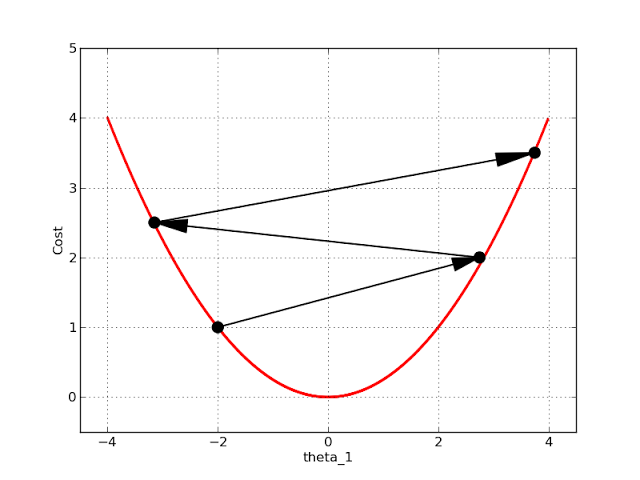
\includegraphics[width = 1.5in]{/home/secondmath/Dropbox/GSPH/topic_review/DNN/hy4.png}} 
\end{figure}
\end{frame}

\begin{frame}{Example\citep{perceptroncant}}
\begin{figure}
\centering
\includegraphics[width=4.5in,page=6]{/home/secondmath/Dropbox/GSPH/topic_review/DNN/lec3.pdf}
\end{figure}
\end{frame}

\begin{frame}
\begin{figure}
\centering
\includegraphics[width=4.5in,page=7]{/home/secondmath/Dropbox/GSPH/topic_review/DNN/lec3.pdf}
\end{figure}
\end{frame}

\begin{frame}
\begin{figure}
\centering
\includegraphics[width=4.5in,page=8]{/home/secondmath/Dropbox/GSPH/topic_review/DNN/lec3.pdf}
\end{figure}
\end{frame}

\begin{frame}
\begin{figure}
\centering
\includegraphics[width=4.5in,page=9]{/home/secondmath/Dropbox/GSPH/topic_review/DNN/lec3.pdf}
\end{figure}
\end{frame}

\begin{frame}
\begin{figure}
\centering
\includegraphics[width=4.5in,page=10]{/home/secondmath/Dropbox/GSPH/topic_review/DNN/lec3.pdf}
\end{figure}
\end{frame}

\begin{frame}{Backpropagation Algorithm\citep{kimjunmoppt}}
\begin{figure}
\subfloat[Forward Propagation]{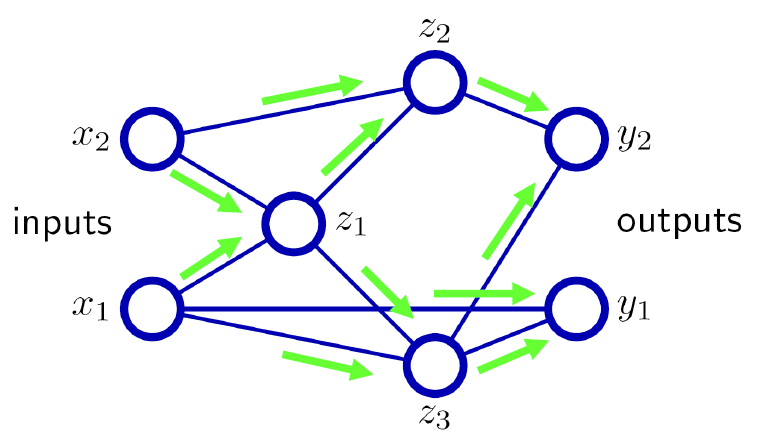
\includegraphics[width = 2.2in]{/home/secondmath/Dropbox/GSPH/topic_review/DNN/forward.png}} 
\subfloat[Back Propagation]{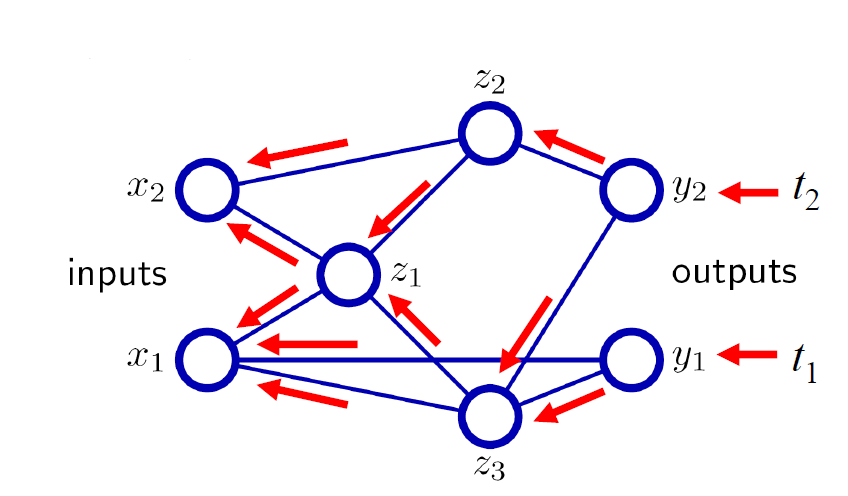
\includegraphics[width = 2.2in]{/home/secondmath/Dropbox/GSPH/topic_review/DNN/back.png}}
\end{figure}
\end{frame}

\begin{frame}{Limitations of MLP\citep{kimjunmoppt}}
\begin{enumerate}
\item \textbf{Vanishing gradient} problem
\item Typically requires lots of \textbf{labeled data}
\item \textbf{Overfitting} problem: Given limited amounts of labeled data, training via back-propagation does not work well
\item Get stuck in \textbf{local minima} (?)
\end{enumerate} 
\end{frame}

\begin{frame}{Vanishing Gradient\citep{bengio1994learning}}
\begin{figure}[!ht]
\centering
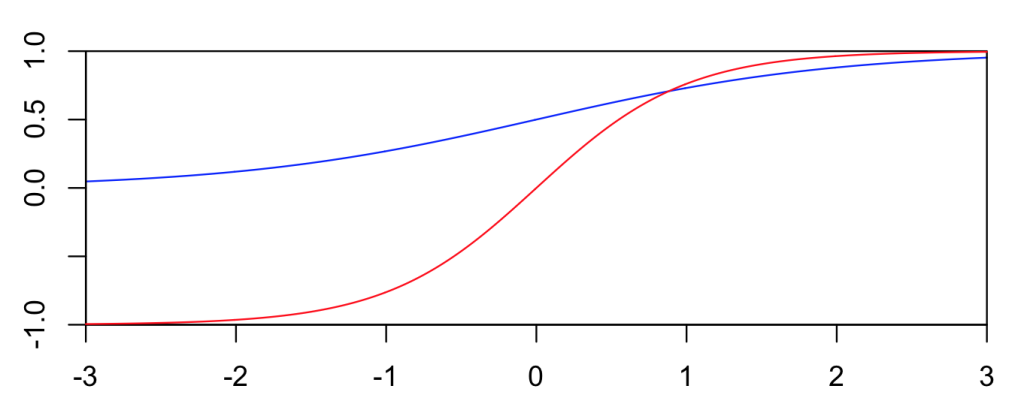
\includegraphics[width=4in]{/home/secondmath/Dropbox/GSPH/topic_review/DNN/logistictan.png}
\caption{\bf{Sigmoid functions}}
\end{figure}
\end{frame}

\begin{frame}{Local Minima\citep{kimjunmoppt}}
\begin{figure}[!ht]
\centering
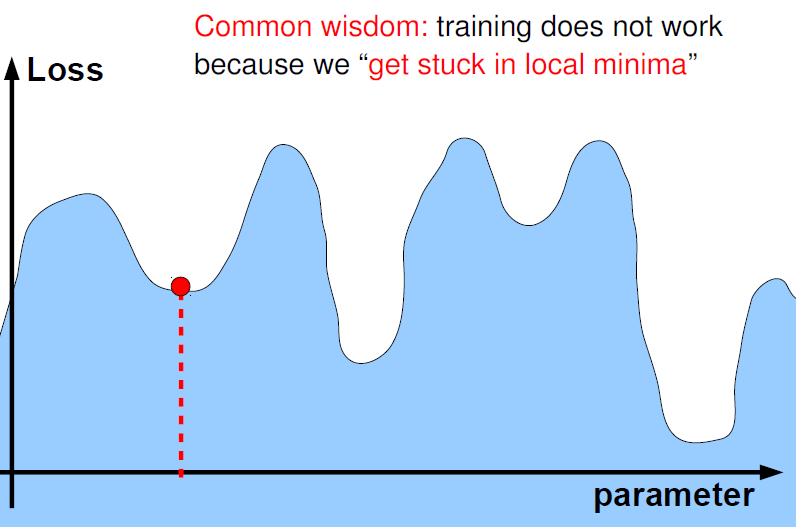
\includegraphics[width=4in]{/home/secondmath/Dropbox/GSPH/topic_review/DNN/minima.png}
\caption{\bf{Global and Local Minima}}
\label{minima}
\end{figure}
\end{frame}




\subsection{1st Breakthrough: Unsupervised Learning}
\begin{frame}{1st Breakthrough: Unsupervised Learning}
2006년 \textbf{Restricted Boltzmann Machine}, Deep Belief Network, Deep Boltzmann Machine\citep{smolensky1986information,hinton2006reducing}..
\begin{figure}[!ht]
\centering
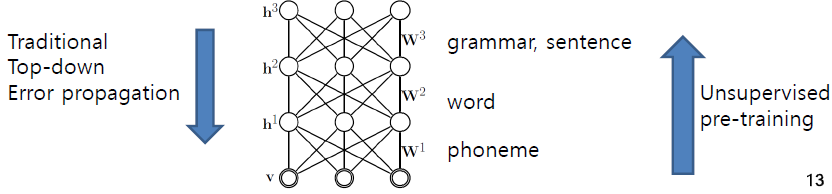
\includegraphics[width=4in]{/home/secondmath/Dropbox/GSPH/topic_review/DNN/unsupervised.png}
\label{unsupervised}
\caption{\bf{Description of Unsupervised Learning}\citep{kimjunmoppt}}
\end{figure}
\end{frame}


\begin{frame}{Limitations of MLP\citep{kimjunmoppt}}
\begin{enumerate}
\item \textbf{Vanishing gradient} problem
\begin{itemize}
  \item \textcolor{red}{Solved by bottom-up layerwise unsupervised pre-training}
\end{itemize}
\item Typically requires lots of \textbf{labeled data}
\item \textbf{Overfitting} problem: Given limited amounts of labeled data, training via back-propagation does not work well
\begin{itemize}
  \item \textcolor{red}{Solved by using lots of unlabeled data}
\end{itemize}
\item Get stuck in \textbf{local minima} (?)
\begin{itemize}
  \item \textcolor{red}{Unsupervised pre-training may help the network initialize with good parameters}
\end{itemize}
\end{enumerate} 
\end{frame}

\begin{frame}{Restricted Boltzmann Machine(RBM)}
\textbf{에너지가 낮을수록 확률이 높다}
\begin{align*}
P(v,h)=\frac{1}{Z}\exp^{-E(v,h)}
\end{align*}
(Z: Normalized Constant)\\
\begin{figure}[!ht]
\centering
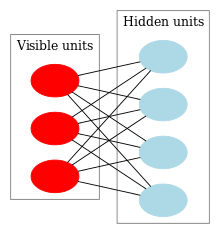
\includegraphics[width=1.5in]{/home/secondmath/Dropbox/GSPH/topic_review/DNN/RBM.png}
\caption{\bf{Diagram of a Restricted Boltzmann\citep{RBMfigure}}}
\end{figure}
\end{frame}

\begin{frame}{Energy Function}
\begin{align*}
E(v,h)= -\sum_i a_i v_i - \sum_j b_j h_j -\sum_i \sum_j h_j w_{i,j} v_i=-a^{\mathrm{T}} v - b^{\mathrm{T}} h -h^{\mathrm{T}} W v
\end{align*}
($a_i$: offset of visible variable, $b_j$: offset of hidden variable, $w_{i,j}$: weight between $v_i$ and $h_j$)
\end{frame}

\begin{frame}{목표}
\textbf{$P(v)=\sum_h P(v,h)$를 최대화 하는 $v$와 그때의 weight들을 구하는 것.}

\begin{align*}
E(v,h)= -\sum_i a_i v_i - \sum_j b_j h_j -\sum_i \sum_j h_j w_{i,j} v_i=-a^{\mathrm{T}} v - b^{\mathrm{T}} h -h^{\mathrm{T}} W v
\end{align*}
\begin{itemize}
  \item 즉, \textbf{$h$, $v$가 동시에 켜진 쪽의 weight를 크게하려는 의도}
  \item 같이 활성화되는 시냅스(synapse)는 연결된다. 
\end{itemize}
\end{frame}

\begin{frame}{Hebb’s Law (Hebbian Learning Rule)}
\begin{figure}
\subfloat{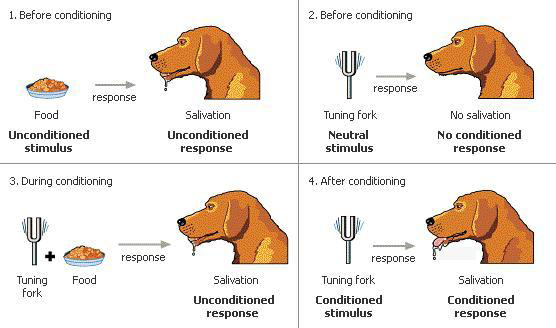
\includegraphics[width = 2.2in]{/home/secondmath/Dropbox/GSPH/topic_review/DNN/dog.png}} 
\subfloat{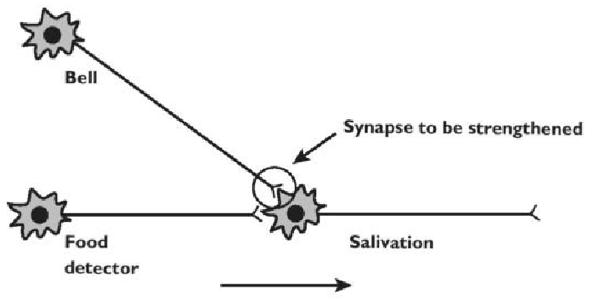
\includegraphics[width = 2.2in]{/home/secondmath/Dropbox/GSPH/topic_review/DNN/dog2.png}}
\end{figure}
\url{http://www.skewsme.com/behavior.htm}\\ \url{http://lesswrong.com/lw/71x/a_crash_course_in_the_neuroscience_of_human/l}
\end{frame}

\begin{frame}{Traing RBM}
$P(v)=\sum_h P(v,h)$를 \textbf{최대화} 하는 $v$와 그때의 weight들을 구하는 것.
\begin{itemize}
  \item \textbf{Gradient Ascent} 
\end{itemize}
\begin{subequations}
\begin{align*}
logP(v)&=log(\sum_{h} \frac{\exp^{-E(v,h)}}{Z})\\
&=log(\sum_h \exp^{-E(v,h)})-logZ\\
&=log(\sum_h \exp^{-E(v,h)})-log(\sum_{v,h} \exp^{-E(v,h)})
\end{align*}
\end{subequations}
\end{frame}

\begin{frame}\tiny
\begin{subequations}
 \label{RBMdiff}
 \begin{align*}
  \frac{\partial logP(v)}{\partial \theta}&=-\frac{1}{\sum_h \exp^{-E(v,h)}} \sum_h \exp^{-E(v,h)}\frac{\partial E(v,h)}{\partial \theta}+\frac{1}{\sum_{v,h} \exp^{-E(v,h)}} \sum_{v,h} \exp^{-E(v,h)}\frac{\partial E(v,h)}{\partial \theta} \\
  &= -\sum_{h} p(h|v) \frac{\partial E(v,h)}{\partial \theta} + \sum_{v,h} p(h,v)\frac{\partial E(v,h)}{\partial \theta} 
 \end{align*}
\end{subequations}
\end{frame}

\begin{frame}
\begin{subequations}
 \begin{align*}
  P(v|h) = \prod_{i=1}^m P(v_i|h)  \\
  P(h|v) = \prod_{j=1}^n P(h_j|v) 
 \end{align*}
\end{subequations}
\begin{subequations}
 \begin{align*}
  p(h_j=1|v) = \sigma \left(b_j + \sum_{i=1}^m w_{i,j} v_i \right)\\
  p(v_i=1|h) = \sigma \left(a_i + \sum_{j=1}^n w_{i,j} h_j \right)
 \end{align*}
\end{subequations}
($\sigma$: activation function)
\end{frame}


\begin{frame}
\begin{align*}
\frac{\partial logP(v)}{\partial \theta}=-\sum_{h} p(h|v) \frac{\partial E(v,h)}{\partial \theta} + \sum_{v,h} p(h,v)\frac{\partial E(v,h)}{\partial \theta} 
\end{align*}
변형된 Gibbs sampler로 Sampling하여 해결 
\end{frame}


\begin{frame}
\begin{figure}[!ht]
\centering
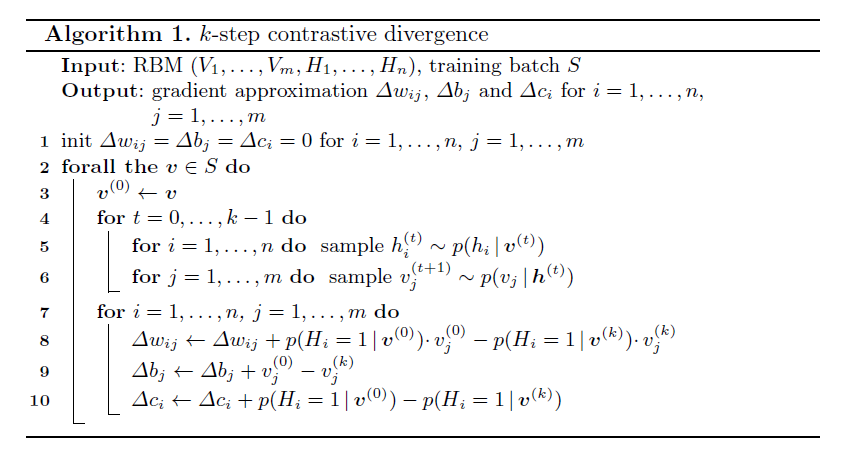
\includegraphics[width=4in]{/home/secondmath/Dropbox/GSPH/topic_review/DNN/cdk.png}
\caption{\bf{Contrastive Divergence(CD-$k$)\citep{fischer2012introduction}}}
\label{cdk}
\end{figure}
\end{frame}

\begin{frame}{Deep Belief Network\citep{hinton2006fast,hinton2009deep,bengio2009learning}}
\begin{enumerate}
  \item Multiple RBM
  \item Phoneme $\rightarrow$ Word $\rightarrow$ Grammer, Sentence
  \item Generation도 가능!!! 
\end{enumerate}
\begin{figure}[!ht]
\centering
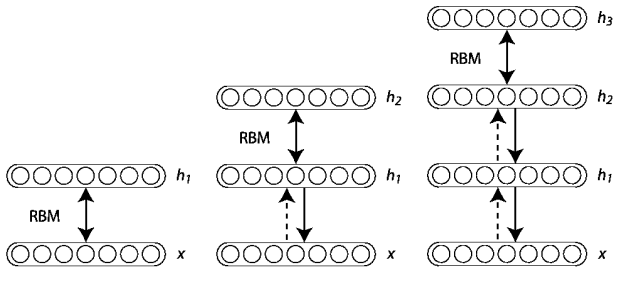
\includegraphics[width=3in]{/home/secondmath/Dropbox/GSPH/topic_review/DNN/dbn2.png}
\end{figure}
 \url{http://www.cs.toronto.edu/~hinton/adi/index.htm}
\end{frame}


\subsection{2nd Breakthrough: Supervised Learning} 
\begin{frame}{2nd Breakthrough: Supervised Learning}
\begin{enumerate}
\item \textbf{Vanishing gradient} problem
\begin{itemize}
  \item Solved by a new non-linear activation :\textcolor{red}{rectified linear unit (ReLU)}
\end{itemize}
\item Typically requires lots of \textbf{labeled data}
\begin{itemize}
  \item Solved by \textcolor{red}{big data} \& crowd sourcing
\end{itemize}
\item \textbf{Overfitting} problem: Given limited amounts of labeled data, training via back-propagation does not work well
\begin{itemize}
  \item Solved by a \textcolor{red}{new regularization method : dropout, dropconnect}, etc
\end{itemize}
\item Get stuck in \textbf{local minima} (?)
\end{enumerate} 
\end{frame}

\begin{frame}{Rectified Linear Unit (ReLU)}
\begin{figure}[!ht]
\centering
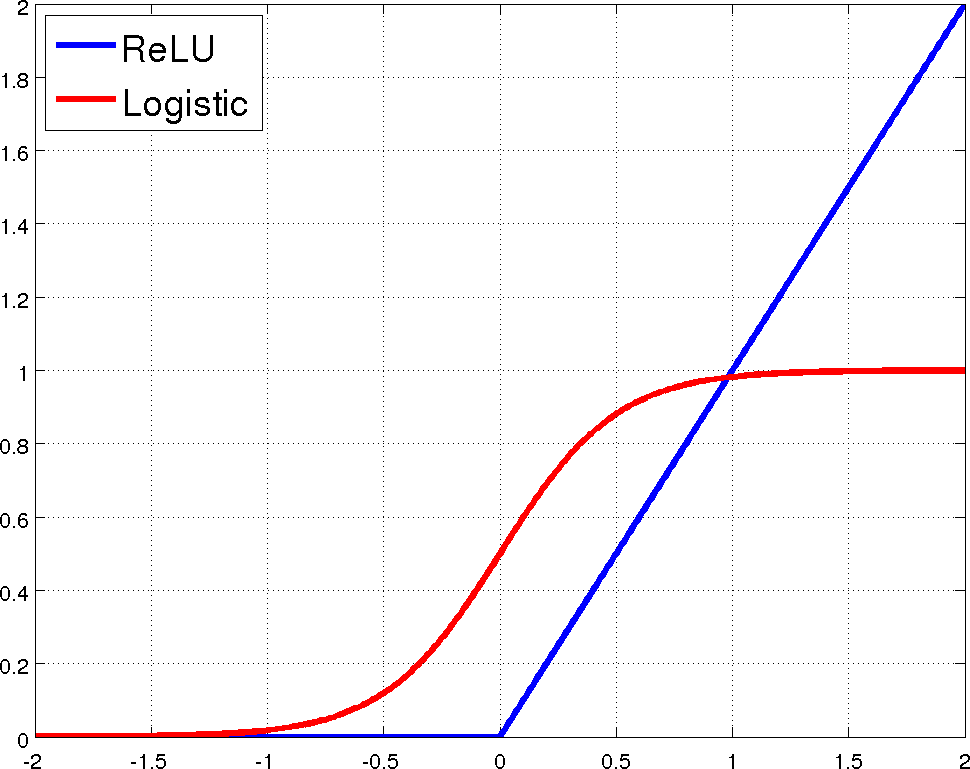
\includegraphics[width=3in]{/home/secondmath/Dropbox/GSPH/topic_review/DNN/relu.png}
\caption{\bf{The proposed non-linearity, ReLU, and the standard neural network non-linearity, logistic\citep{zeiler2013rectified}}}
\end{figure}
\end{frame}

\begin{frame}{장점}
\begin{enumerate}
  \item 0보다만 크면 항상 기울기가 1로 일정해 기울기가 감소하는 경우가 없다. 
  \item 학습이 쉽다. 
  \item Pre-training의 필요성을 없애준다.\citep{nair2010rectified,glorot2011deep}.
\end{enumerate}
\end{frame}

\begin{frame}{DropOut \& DropConnect}
\textbf{Ensemble Model}
\begin{itemize}
  \item \textbf{DropOut}: hidden unit의 일부를 쉬게 한다\citep{hinton2012improving}. 
  \item \textbf{DropConnect}: hidden unit으로의 연결 중 일부를 쉬게 한다\citep{wan2013regularization}. 
\end{itemize}
\end{frame}

\begin{frame}
\begin{figure}[!ht]
\centering
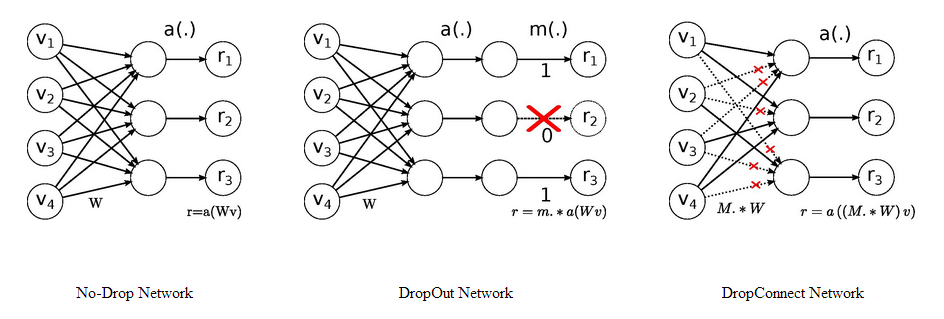
\includegraphics[width=4in]{/home/secondmath/Dropbox/GSPH/topic_review/DNN/dropout.png}
\caption{\bf{Description of DropOut \& DropConnect\citep{dropfig}}}
\end{figure}
\end{frame}

\begin{frame}
\begin{figure}[!ht]
\centering
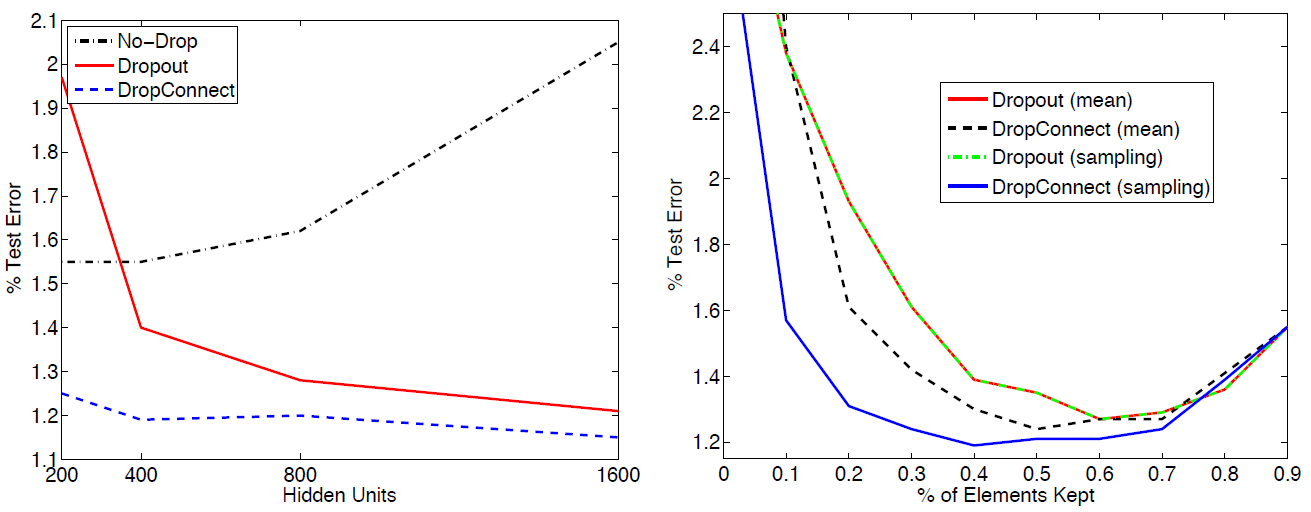
\includegraphics[width=4in]{/home/secondmath/Dropbox/GSPH/topic_review/DNN/dropperformance.png}
\caption{\bf{Using the MNIST dataset, in a) Ability of Dropout and DropConnect to prevent overfitting as the size of the 2 fully connected layers increase. b) Varying the drop-rate in a 400-400 network shows near optimal performance around the $p$ = 0.5\citep{wan2013regularization}}}
\label{dropperformance}
\end{figure}
\end{frame}

\begin{frame}{Local Minima Issue}
\textbf{High dimension and non-convex optimization} 
\begin{enumerate}
  \item Local minima들의 값이 비슷비슷할 것
  \item Local minima $\simeq$ Global minima. 
  \item 수많은 차원에서 차원마다 local minima이기는 어렵다.  
\end{enumerate}
\end{frame}

\begin{frame}
\begin{figure}[!ht]
\centering
\includegraphics[width=4in,page=31]{/home/secondmath/Dropbox/GSPH/topic_review/DNN/ranzato.pdf}
\caption{\bf{Local minima when high dimension and non-convex optimization \citep{minima}}}
\end{figure}
\end{frame}



\begin{frame}{Others: Convolutional Neural Network}
\textbf{Sparse Connectivity \& Shared Weight: 2차원 데이터에 적합}\citep{convol}
\begin{figure}[!ht]
\centering
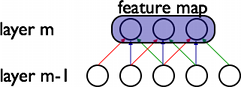
\includegraphics[width=3in]{/home/secondmath/Dropbox/GSPH/topic_review/DNN/conv_1D_nn.png}
\end{figure}
\end{frame}

\begin{frame}
\begin{figure}[!ht]
\centering
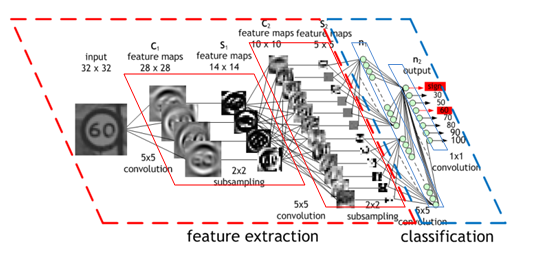
\includegraphics[width=5in]{/home/secondmath/Dropbox/GSPH/topic_review/DNN/con2.png}
\end{figure}
\url{http://parse.ele.tue.nl/education/cluster0}
\end{frame}


\begin{frame}
\begin{figure}
\subfloat{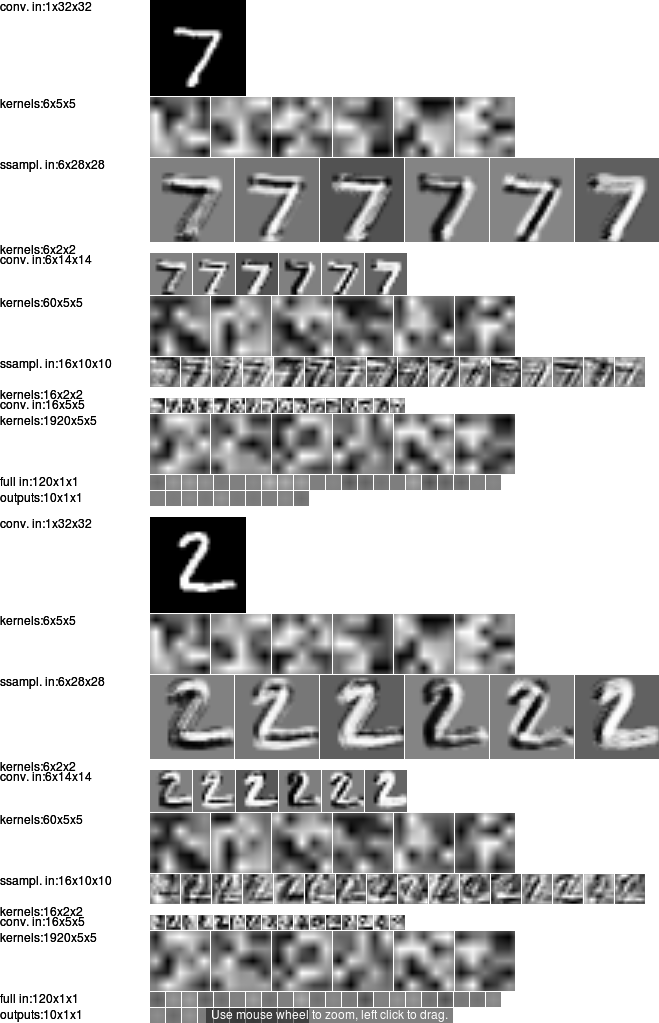
\includegraphics[width = 1.5in]{/home/secondmath/Dropbox/GSPH/topic_review/DNN/mnist_fprop0.png}} 
\subfloat{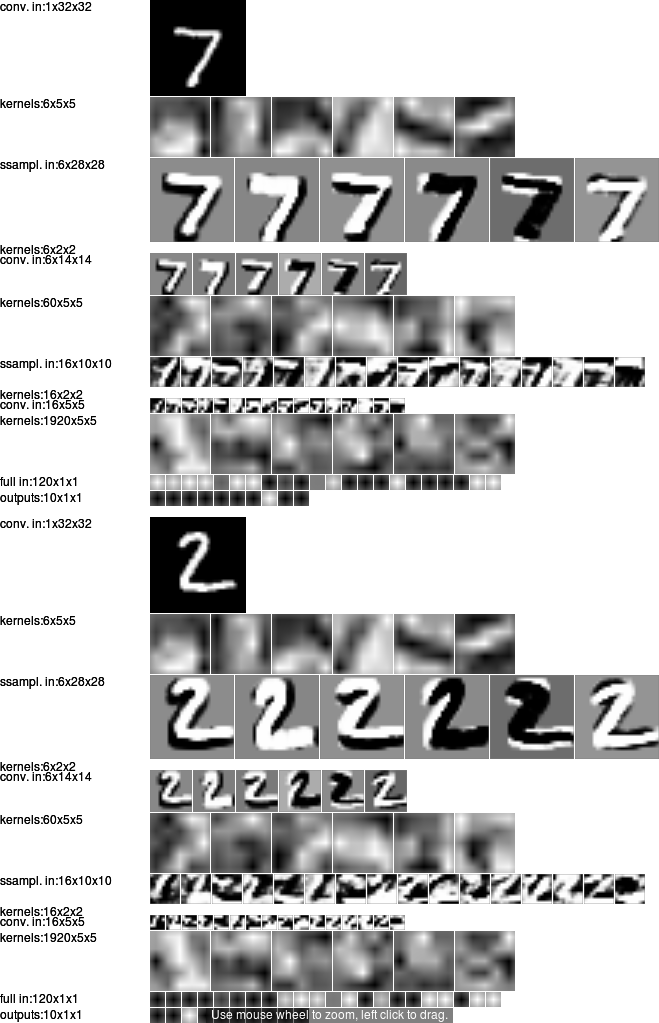
\includegraphics[width = 1.5in]{/home/secondmath/Dropbox/GSPH/topic_review/DNN/mnist_fprop1.png}}
\end{figure}
\url{http://eblearn.sourceforge.net/old/demos/mnist/index.shtml}\\ \url{http://yann.lecun.com/exdb/lenet/}
\end{frame}



\begin{frame}{Deep Learning Summary!!!}\footnotesize
\begin{enumerate}
  \item 1950년대 \textbf{퍼셉트론(perceptron)}에서 시작된 인공신경망 연구는 1980년대 \textbf{오류역전파알고리즘(Error Backpropagation Algorithm)}으로 다층퍼셉트론(Multilayer perceptron)을 학습할 수 있게 되면서 발전.
  \item Gradient vanishing, labeled data의 부족, overfitting, local minima issue 등이 잘 해결되지 못해 2000년대 초까지 인공신경망 연구는 답보상태.
  \item 2006년부터 \textbf{볼츠만머신을 이용한 Unsupervised Learning}인 Restricted Boltzmann Machine(RBM), Deep Belief Network(DBN), Deep Boltzmann Machine(DBM), Convolutional Deep Belief Network 등이 개발.
  \item Unlabeled data를 이용하여 pre-training을 수행할 수 있게 되어 위에 언급된 다층퍼셉트론의 한계점이 극복됨.
  \item 2010년부터는 빅데이터를 적극적으로 이용함으로서 수많은 labeled data를 사용할 수 있게 되었고, \textbf{Rectified linear unit (ReLU), DropOut, DropConnect} 등의 발견으로 vanishing gradient문제와 overfitting issue를 해결하여 아예 \textbf{Supervised learning}이 가능.
  \item Local minima issue는 High dimension non-convex optimization에서는 별로 중요한 부분이 아니라는 공감대.
  \end{enumerate}
\end{frame}



\section{\protect\textbf{Apply to Public Health}}

\subsection{Epidemiology vs Machine Learning}

\begin{frame}{Objective of statistics}
\begin{enumerate}
\item 지식의 확장, Causal inference
\begin{itemize}
\item 통계학자 Pearson: 다윈의 진화론 증명을 위하여..
\end{itemize}
\item 의사결정
\begin{itemize}
\item 통계학자 R.A Fisher: 가장 성능이 좋은 비료 선택 
\end{itemize}
\end{enumerate}
\end{frame}

\begin{frame}{Statistics in Epidemiology}
\begin{itemize}
\item Causal inference: 원인이 무엇인가? 
\item 해석이 잘되는 모형이 짱이다. 인과관계 추론. 
\item 간단한 모형 선호. 
\item 독립변수의 단위도 중요(Kilometer VS meter, centering issue)
\item \bf{$\beta$}, \textbf{Odds Ratio(OR), Hazard Ratio(HR), p-value}, \bf{$AIC$}
\end{itemize}
\end{frame}

\begin{frame}{Statistics in Machine Learning}
\begin{itemize}
\item Prediction: 앞으로 어떻게 될 것인가? 
\item 예측력이 좋은 것이 짱이다.  
\item 복잡한 모형도 상관없다. 예측만 효율적으로 잘 한다면. 
\item 필요에 따라 독립변수들을 자유자재로 바꾼다. (Scale change)
\item \bf{$\hat{Y}$}, \bf{$\hat{p}$}, \textbf{Cross-validation, Accuracy, ROC curve}
\end{itemize}
\end{frame}

\begin{frame}{Example: Logistic regression}
\begin{itemize}
\item Binomial data를 다루는 강력한 통계분석방법. 
\item 특히 epidemiologic study에서는 절대적인 지위.
\item $\beta \rightarrow \text{Odds Ratio(OR)}$ : \textbf{해석이 쉽다.} 
\end{itemize}
\textbf{But..}
\begin{itemize}
\item Logit function... 계산이 어려워지는 원인.
\item Heritability issue of binomial trait?? Logit함수가 범인..
\item Probit model이 대안이 될 수 있다. 
 \begin{itemize}
 \item 계산쉽다. 
 \item $\beta$ 해석 어렵다..
 \end{itemize}
\end{itemize}
\end{frame}

\begin{frame}{Logit VS Probit}
\begin{figure}
\includegraphics[width=2.5in]{/home/secondmath/Dropbox/GSPH/myreview/ml/probit.png}
\caption{Logit VS Probit}
\end{figure}
\begin{itemize}
\item Logit: $\Pr(Y=1 \mid X) = [1 + e^{-X'\beta}]^{-1}$
\item Probit: $\Pr(Y=1 \mid X) = \Phi(X'\beta)$
\end{itemize}
\end{frame}





\begin{frame}{Example2: Cox proportional hazard model}
\textbf{Censored data분석의 표준.}
\begin{figure}
\includegraphics[width=2.5in]{/home/secondmath/Dropbox/GSPH/myreview/ml/censored.jpg}
\end{figure}
\url{http://www.theriac.org/DeskReference/viewDocument.php?id=188}
\end{frame}


\begin{frame}
\begin{figure}
\includegraphics[width=2.5in]{/home/secondmath/Dropbox/GSPH/myreview/ml/cox.png}
\end{figure}
\url{http://www.uni-kiel.de/psychologie/rexrepos/posts/survivalCoxPH.html}
\end{frame}

\begin{frame}{Assumptions}
\begin{equation*}
\begin{array}{rclcl}
\ln \lambda(t) &=& \ln \lambda_{0}(t) + \beta_{1} X_{1} + \dots + \beta_{p} X_{p}      &=& \ln \lambda_{0}(t) + \bf{X} \bf{\beta}\\
    \lambda(t) &=&     \lambda_{0}(t) \, e^{\beta_{1} X_{1} + \dots + \beta_{p} X_{p}} &=& \lambda_{0}(t) \, e^{\bf{X} \bf{\beta}}\\
S(t)           &=& S_{0}(t)^{\exp(\bf{X} \bf{\beta})} &=& \exp\left(-\Lambda_{0}(t) \, e^{\bf{X} \bf{\beta}}\right)\\
\Lambda(t)     &=& \Lambda_{0}(t) \, e^{\bf{X} \bf{\beta}} & &
\end{array}
\end{equation*}
\begin{equation*}
\frac{\lambda(t)}{\lambda_{0}(t)}=e^{\bf{X} \bf{\beta}}
\end{equation*}
\bf{$\beta$} : \textbf{Hazard Ratio(HR)}
\end{frame}

\begin{frame}{Hazard Ratio}
\begin{itemize}
\item 해석 편하다. Odd Ratio 급. 
\item \textbf{But, } 가정이 많이 들어간다. 
\item 식이 복잡해서 계산이 어렵다. 
\item Conditional Logistic Regression.. 
\item \textbf{Prediction에도 Cox를 고집할 필요는 없다.}
\end{itemize}
\end{frame}

\begin{frame}{Alternatives}
$\bf{Y_i}$ : \textbf{Time of event}
\begin{block}{Not censored}
\begin{equation*}
p(y_i|\mu_i,\sigma^2)=(2\pi\sigma^2)^{-\frac{1}{2}}exp{\{-\frac{(y_i-\mu_i)^2}{2\sigma^2}\}}
\end{equation*}
\end{block}

\begin{block}{Censored}
\begin{equation*}
p(y_i\ge t_i|\mu_i,\sigma^2)=\int_{t_i}^{\infty}(2\pi\sigma^2)^{-\frac{1}{2}}exp{\{-\frac{(y_i-\mu_i)^2}{2\sigma^2}\}}\partial y_i=\Phi{(\frac{\mu_i-t_i}{\sigma})}
\end{equation*}
\end{block}
정규분포의 CDF로 간단히 표현 $\rightarrow$ \textbf{계산이 쉽다!!} 
\end{frame}

\begin{frame}{Example3: Correlation Structure}
\textbf{Correlation structure 고려해야하나?} 
\begin{enumerate}
\item Epidemiology: \textbf{Important}
 \begin{itemize}
  \item $\beta$의 s.e가 바뀐다. $\rightarrow$ \textbf{p-value가 바뀐다}.
 \end{itemize}
\item Prediction model: \textbf{Not important}
 \begin{itemize}
  \item $\beta$ 자체는 크게 안바뀐다.$\rightarrow$ $\hat{Y}, \hat{p}$는 잘 안바뀐다.  
  \item Correlation structure : \textbf{Unmeasured} effect $\rightarrow$ 측정되지 않은 것은 New data에서 prediction할 때 이용할 수 없다.  
 \end{itemize}
\end{enumerate}
\end{frame}




\begin{frame}
\begin{figure}
\includegraphics[width=3.5in]{/home/secondmath/Dropbox/GSPH/myreview/ml/interpretation.png}
\caption{A representation of the tradeoff between flexibility and interpretability,
using different statistical learning methods. In general, as the flexibility
of a method increases, its interpretability decreases\citep{james2013introduction}}
\end{figure}
\end{frame}


\begin{frame}
\begin{figure}
\includegraphics[width=2.5in]{/home/secondmath/Dropbox/GSPH/myreview/ml/ted.pdf}
\end{figure}
\end{frame}

\begin{frame}{Human VS metahuman\citep{chiang2000catching}}
\textbf{Ted Chiang} : SF 소설가 
\begin{itemize}
\item 메타 인류(인공지능)의 압도적인 지식처리능력. 
\item Human science: 메타 인류가 밝혀낸 것들을 해석하는 정도의 수준. 
\item 메타 인류의 논문을 번역하는 것이 human science..
\end{itemize}
\end{frame}


\subsection{Deep Learning vs Other ML}
\begin{frame}{Deep Learning vs Other ML}
\begin{itemize}
  \item Multiple Hidden Layer: High flexibility
  \item \textbf{Massive Parallel Computing}
\end{itemize}

\begin{itemize}
  \item Programming language for GPU/parallel computing
  \item \textbf{ CUDA(Compute Unified Device Architecture), OpenCL}\citep{nvidia2007compute,stone2010opencl}
\end{itemize}
\end{frame}


\begin{frame}{Examples: Cat recognition}
\begin{itemize}
\item 16,000개의 CPU
\item 그림만 보고 고양이 인식 (Unsupervised Learning)
\item GPU를 이용하여 Computing 시간 줄임. 
\end{itemize}
\url{http://www.asiae.co.kr/news/view.htm?idxno=2012062708351993171}
\url{http://googleblog.blogspot.kr/2012/06/using-large-scale-brain-simulations-for.html}
\end{frame}


\begin{frame}{Paper\citep{le2013building,coates2013deep}}
\begin{figure}
\centering
\subfloat{\includegraphics[width=.5\textwidth,page=1]{/home/secondmath/Dropbox/GSPH/myreview/ml/unsupervised_icml2012.pdf}} 
\subfloat{\includegraphics[width=.5\textwidth,page=1]{/home/secondmath/Dropbox/GSPH/myreview/ml/CoatesHuvalWangWuNgCatanzaro_icml2013.pdf}}
\end{figure}
\end{frame}



\subsection{Hypothesis Testing vs Hypothesis Generating}

\begin{frame}{Hypothesis Testing vs Hypothesis Generating}
\begin{figure}
\includegraphics[width=4.5in]{/home/secondmath/Dropbox/GSPH/myreview/journalreview/textmining6.png}
\caption{\bf{Hypothesis-testing and Hypothesis-generating
paradigms\citep{biesecker2013hypothesis}}}
\end{figure}
\end{frame}

\begin{frame}
\begin{figure}
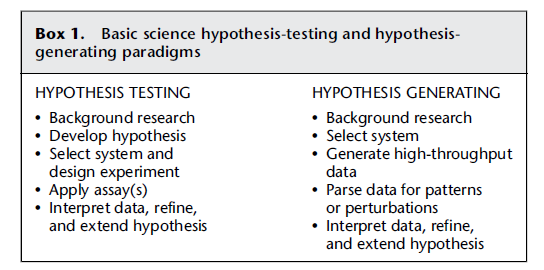
\includegraphics[width=4in]{/home/secondmath/Dropbox/GSPH/myreview/journalreview/textmining7.png}
\end{figure}
\end{frame}


\begin{frame}
\begin{figure}
\includegraphics[width=4in]{/home/secondmath/Dropbox/GSPH/myreview/journalreview/textmining8.png}
\end{figure}
\end{frame}


\begin{frame}
\begin{figure}
\includegraphics[width=4in]{/home/secondmath/Dropbox/GSPH/myreview/journalreview/textmining9.png}
\end{figure}
\end{frame}

\section{\protect\textbf{Conclusion}}
\begin{frame}{Conclusion}
\textbf{Deep Learning이 Mobile Health 의 핵심}.
\begin{itemize}
  \item Mobile data: 영상, 음성, 텍스트 등 비정형 데이터. 
  \item Parallel Computing System 구축이 필요하다. 
\end{itemize}
\textbf{Prediction vs Inference}
\begin{itemize}
  \item Understanding concept of Machine Learning
  \item Hypothesis Generating
  \item Paradigm shift: Causal inference $\rightarrow$ Big data \& Prediction
\end{itemize}
\end{frame}





\begin{frame}[allowframebreaks]{Reference}\tiny
\bibliographystyle{apalike}
\bibliography{DNN}
\end{frame}



\end{document}

